\documentclass{standalone}
\usepackage{tikz}
\usetikzlibrary{patterns, positioning}


\begin{document}
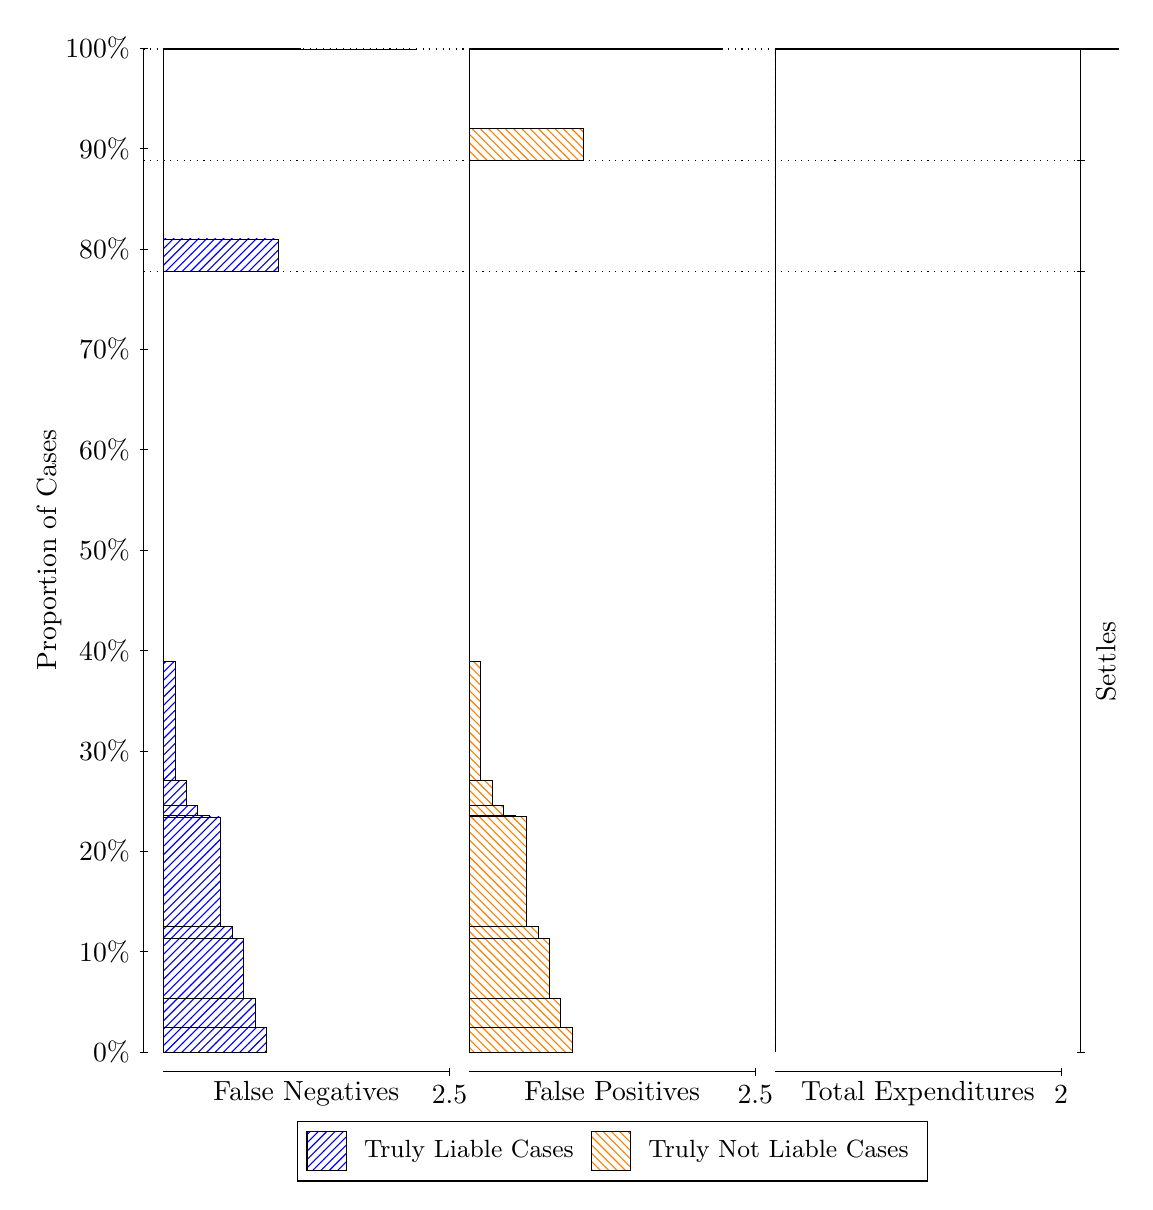
\begin{tikzpicture}
\draw[black, very thin] (1.5,1.75) -- (1.5,14.5);
\node[rotate=90, text=black, anchor=center] at (0.3, 8.125) {Proportion of Cases};
\draw[black, very thin] (1.45,1.75) -- (1.55,1.75);
\node[text=black, anchor=east] at (1.45, 1.75) {0\%};
\draw[black, very thin] (1.45,3.025) -- (1.55,3.025);
\node[text=black, anchor=east] at (1.45, 3.025) {10\%};
\draw[black, very thin] (1.45,4.3) -- (1.55,4.3);
\node[text=black, anchor=east] at (1.45, 4.3) {20\%};
\draw[black, very thin] (1.45,5.575) -- (1.55,5.575);
\node[text=black, anchor=east] at (1.45, 5.575) {30\%};
\draw[black, very thin] (1.45,6.85) -- (1.55,6.85);
\node[text=black, anchor=east] at (1.45, 6.85) {40\%};
\draw[black, very thin] (1.45,8.125) -- (1.55,8.125);
\node[text=black, anchor=east] at (1.45, 8.125) {50\%};
\draw[black, very thin] (1.45,9.4) -- (1.55,9.4);
\node[text=black, anchor=east] at (1.45, 9.4) {60\%};
\draw[black, very thin] (1.45,10.675) -- (1.55,10.675);
\node[text=black, anchor=east] at (1.45, 10.675) {70\%};
\draw[black, very thin] (1.45,11.95) -- (1.55,11.95);
\node[text=black, anchor=east] at (1.45, 11.95) {80\%};
\draw[black, very thin] (1.45,13.225) -- (1.55,13.225);
\node[text=black, anchor=east] at (1.45, 13.225) {90\%};
\draw[black, very thin] (1.45,14.5) -- (1.55,14.5);
\node[text=black, anchor=east] at (1.45, 14.5) {100\%};

\draw[black, very thin] (13.4,1.75) -- (13.4,14.5);
\draw[black, very thin] (13.35,1.75) -- (13.45,1.75);
\node[anchor=west] at (13.35, 1.75) {};
\draw[black, very thin] (13.35,11.665) -- (13.45,11.665);
\node[anchor=west] at (13.35, 11.665) {};
\draw[black, very thin] (13.35,13.072) -- (13.45,13.072);
\node[anchor=west] at (13.35, 13.072) {};
\draw[black, very thin] (13.35,14.48) -- (13.45,14.48);
\node[anchor=west] at (13.35, 14.48) {};
\draw[black, very thin] (13.35,14.49) -- (13.45,14.49);
\node[anchor=west] at (13.35, 14.49) {};
\draw[black, very thin] (13.35,14.5) -- (13.45,14.5);
\node[anchor=west] at (13.35, 14.5) {};

\draw[black, very thin, pattern color=blue, pattern=north east lines] (1.75,1.75) rectangle (3.058,2.0671);
\draw[black, very thin, pattern color=blue, pattern=north east lines] (1.75,2.0671) rectangle (2.9127,2.4276);
\draw[black, very thin, pattern color=blue, pattern=north east lines] (1.75,2.4276) rectangle (2.7673,3.1886);
\draw[black, very thin, pattern color=blue, pattern=north east lines] (1.75,3.1886) rectangle (2.622,3.3414);
\draw[black, very thin, pattern color=blue, pattern=north east lines] (1.75,3.3414) rectangle (2.4767,4.737);
\draw[black, very thin, pattern color=blue, pattern=north east lines] (1.75,4.737) rectangle (2.3313,4.7512);
\draw[black, very thin, pattern color=blue, pattern=north east lines] (1.75,4.7512) rectangle (2.186,4.8861);
\draw[black, very thin, pattern color=blue, pattern=north east lines] (1.75,4.8861) rectangle (2.0407,5.1986);
\draw[black, very thin, pattern color=blue, pattern=north east lines] (1.75,5.1986) rectangle (1.8953,6.7073);
\draw[black, very thin, pattern color=orange, pattern=north west lines] (1.75,6.7073) rectangle (1.75,11.665);
\draw[black, very thin, pattern color=blue, pattern=north east lines] (1.75,11.665) rectangle (3.2033,12.075);
\draw[black, very thin, pattern color=orange, pattern=north west lines] (1.75,12.075) rectangle (1.75,13.072);
\draw[black, very thin, pattern color=orange, pattern=north west lines] (1.75,13.072) rectangle (1.75,13.482);
\draw[black, very thin, pattern color=blue, pattern=north east lines] (1.75,13.482) rectangle (1.75,14.48);
\draw[black, very thin, pattern color=blue, pattern=north east lines] (1.75,14.48) rectangle (4.9473,14.483);
\draw[black, very thin, pattern color=orange, pattern=north west lines] (1.75,14.483) rectangle (1.75,14.49);
\draw[black, very thin, pattern color=blue, pattern=north east lines] (1.75,14.49) rectangle (3.494,14.497);
\draw[black, very thin, pattern color=orange, pattern=north west lines] (1.75,14.497) rectangle (1.75,14.5);
\draw[black, very thin, pattern color=orange, pattern=north west lines] (5.6333,1.75) rectangle (6.9413,2.0671);
\draw[black, very thin, pattern color=orange, pattern=north west lines] (5.6333,2.0671) rectangle (6.796,2.4276);
\draw[black, very thin, pattern color=orange, pattern=north west lines] (5.6333,2.4276) rectangle (6.6507,3.1887);
\draw[black, very thin, pattern color=orange, pattern=north west lines] (5.6333,3.1887) rectangle (6.5053,3.3415);
\draw[black, very thin, pattern color=orange, pattern=north west lines] (5.6333,3.3415) rectangle (6.36,4.7371);
\draw[black, very thin, pattern color=orange, pattern=north west lines] (5.6333,4.7371) rectangle (6.2147,4.7513);
\draw[black, very thin, pattern color=orange, pattern=north west lines] (5.6333,4.7513) rectangle (6.0693,4.8862);
\draw[black, very thin, pattern color=orange, pattern=north west lines] (5.6333,4.8862) rectangle (5.924,5.1986);
\draw[black, very thin, pattern color=orange, pattern=north west lines] (5.6333,5.1986) rectangle (5.7787,6.7074);
\draw[black, very thin, pattern color=blue, pattern=north east lines] (5.6333,6.7074) rectangle (5.6333,11.665);
\draw[black, very thin, pattern color=orange, pattern=north west lines] (5.6333,11.665) rectangle (5.6333,12.662);
\draw[black, very thin, pattern color=blue, pattern=north east lines] (5.6333,12.662) rectangle (5.6333,13.072);
\draw[black, very thin, pattern color=orange, pattern=north west lines] (5.6333,13.072) rectangle (7.0867,13.482);
\draw[black, very thin, pattern color=blue, pattern=north east lines] (5.6333,13.482) rectangle (5.6333,14.48);
\draw[black, very thin, pattern color=orange, pattern=north west lines] (5.6333,14.48) rectangle (7.3773,14.487);
\draw[black, very thin, pattern color=blue, pattern=north east lines] (5.6333,14.487) rectangle (5.924,14.49);
\draw[black, very thin, pattern color=orange, pattern=north west lines] (5.6333,14.49) rectangle (8.8307,14.493);
\draw[black, very thin, pattern color=blue, pattern=north east lines] (5.6333,14.493) rectangle (7.3773,14.5);
\draw[black, very thin, pattern color=orange, pattern=north west lines] (9.5167,1.75) rectangle (9.5167,6.7074);
\draw[black, very thin, pattern color=blue, pattern=north east lines] (9.5167,6.7074) rectangle (9.5167,11.665);
\draw[black, very thin, pattern color=orange, pattern=north west lines] (9.5167,11.665) rectangle (9.5167,12.662);
\draw[black, very thin, pattern color=blue, pattern=north east lines] (9.5167,12.662) rectangle (9.5167,13.072);
\draw[black, very thin, pattern color=orange, pattern=north west lines] (9.5167,13.072) rectangle (9.5167,13.482);
\draw[black, very thin, pattern color=blue, pattern=north east lines] (9.5167,13.482) rectangle (9.5167,14.48);
\draw[black, very thin, pattern color=orange, pattern=north west lines] (9.5167,14.48) rectangle (13.877,14.487);
\draw[black, very thin, pattern color=blue, pattern=north east lines] (9.5167,14.487) rectangle (13.877,14.49);
\draw[black, very thin, pattern color=orange, pattern=north west lines] (9.5167,14.49) rectangle (13.877,14.493);
\draw[black, very thin, pattern color=blue, pattern=north east lines] (9.5167,14.493) rectangle (13.877,14.5);
\draw[black, dotted] (1.5,11.665) -- (13.4,11.665);
\draw[black, dotted] (1.5,13.072) -- (13.4,13.072);
\draw[black, dotted] (1.5,14.48) -- (13.4,14.48);
\draw[black, dotted] (1.5,14.49) -- (13.4,14.49);
\draw[black, very thin] (1.75,1.5) -- (5.3833,1.5);
\node[text=black, anchor=north] at (3.5667, 1.5) {False Negatives};
\draw[black, very thin] (5.3833,1.45) -- (5.3833,1.55);
\node[text=black, anchor=north] at (5.3833, 1.45) {2.5};

\draw[black, very thin] (5.6333,1.5) -- (9.2667,1.5);
\node[text=black, anchor=north] at (7.45, 1.5) {False Positives};
\draw[black, very thin] (9.2667,1.45) -- (9.2667,1.55);
\node[text=black, anchor=north] at (9.2667, 1.45) {2.5};

\draw[black, very thin] (9.5167,1.5) -- (13.15,1.5);
\node[text=black, anchor=north] at (11.333, 1.5) {Total Expenditures};
\draw[black, very thin] (13.15,1.45) -- (13.15,1.55);
\node[text=black, anchor=north] at (13.15, 1.45) {2};

\node[text=black, centered, rotate=90] at (13.72, 6.7074) {Settles};





\draw (7.449999999999999,1.5) node[draw=none] (baseCoordinate) {};
\begin{scope}[align=center]
        \matrix[scale=0.5, draw=black, below=0.5cm of baseCoordinate, nodes={draw}, column sep=0.1cm]{
            \node[rectangle, draw, minimum width=0.5cm, minimum height=0.5cm, pattern color=blue, pattern=north east lines] {}; &
            \node[draw=none, font=\small, text=black] (B) {Truly Liable Cases}; &
            \node[rectangle, draw, minimum width=0.5cm, minimum height=0.5cm, pattern color=orange, pattern=north west lines] {}; &
            \node[draw=none, font=\small, text=black] (B) {Truly Not Liable Cases}; \\
            };
\end{scope}

\end{tikzpicture}
\end{document}